\chapter{Background} \label{chap:background}





\section{Properties}

Consider a set of entities $\mathcal{E}$. A formal property $P\subseteq \wp(\mathcal{E}) $ is a set of entities that have this property \cite[chapter 8]{cousot2021}. In the introduction we abstracted the value of a variable, that would be an integer in the concrete, to its sign. With the set of integers as our set of entities $\mathcal{E}=\mathbb{Z}$, a ``positive'' property is defined as $P_{pos}=\{z\in \mathcal{E} \;|\; 0<z\}$ and we can define some more semantic properties like in table \ref{table:properties}.
\begin{table}[hbt]
\begin{center}
  \begin{tabular}{l|l}
  $\mathsf{false}$ & $\emptyset$\\
   $P_{0}$ & $\{0\}$\\
   $P_{pos}$ & $\{z\in \mathbb{Z} \;|\; 0<z\}$\\
   $P_{neg}$ & $\{z\in \mathbb{Z} \;|\; 0>z\}$\\
   $P_{pos0}$ & $\{z\in \mathbb{Z} \;|\; 0\leq z\}$\\
   $P_{neg0}$ & $\{z\in \mathbb{Z} \;|\; 0\geq z\}$\\
   $P_{even}$ & $\{z\in \mathbb{Z} \;|\; \exists k\in\mathbb{Z}:2k=z \}$ \\
   $P_{odd}$ & $\{z\in \mathbb{Z} \;|\; \exists k\in\mathbb{Z}:2k+1=z \}$ \\
   $P_{pos\_even}$ & $\{z\in \mathbb{Z} \;|\; z>0 \wedge \exists k\in\mathbb{Z}:2k=z \} = P_{pos} \cap P_{even}$ \\
   $\vdots$ &$\vdots$\\
   $\mathsf{true}$ & $\mathbb{Z}$\\
  \end{tabular}
  \caption{An incomplete selection of properties for $\mathbb{Z}$.}\label{table:properties}
  \end{center}
\end{table}

\noindent We call a property $P$ ``stronger'' than $P'$ (or $P'$ ``weaker'' than $P$) if $P\subseteq P'$. Its set representation contains less elements and we therefore have more information about an element that fulfils said property. The weakest property is the $\mathsf{true}$ property that is satisfied by alle elements and the strongest is $\mathsf{false}$ which is satisfied by none \cite[chapter 8]{cousot2021}. Not all properties from $\wp(\mathcal{E})$ carry a semantic meaning. We therefore only consider the set of properties of interest $C\subseteq\wp(\mathcal{E})$. If we want to analyse the signs of integers this could be $C_{sign}=\{\mathsf{false}, P_{0}, P_{pos}, P_{neg}, P_{pos0}, P_{neg0}, P_{not0}, \mathsf{true}\}$. The poset  $\langle C,\subseteq\rangle$ is called the ``concrete domain''.

\section{Abstraction}\label{sec:abstraction}

Now consider a set of abstract properties $A$. This is not a power set of concrete values anymore but a set of purely semantic symbols that represent abstract properties. If there exists a Galois connection $\langle C,\subseteq\rangle \galois{\alpha}{\gamma}\langle A\sqsubseteq\rangle$, we call $\langle A\sqsubseteq\rangle$ the abstract domain, $\alpha\in C\to A$ the abstraction function and $\gamma\in A\to C$ the concretisation function \cite[chapter 11]{cousot2021}. To put the working principle of Galois connections into simple terms: $A$'s elements abstract $C$'s elements and $\sqsubseteq$ works analogous in the abstract to $\subseteq$ in the concrete. More formally: $\forall P_C\in C:\forall P_A \in A:\alpha(P_C)\sqsubseteq P_A \Longleftrightarrow P_C \subseteq \gamma(P_A)$.

\begin{figure}[htb]
	\begin{center}
		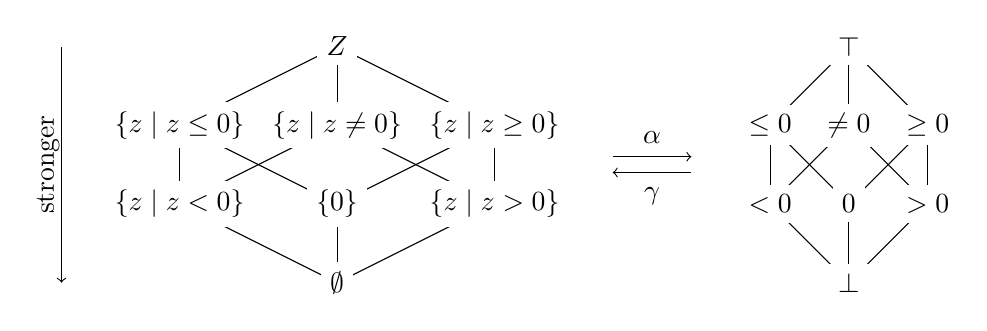
\begin{tikzpicture}
			% Concrete domain
			\draw (-4.5,0) -- (-6.5,1);
            \draw (-4.5,0) -- (-4.5,1);
            \draw (-4.5,0) -- (-2.5,1);
            \draw (-4.5,3) -- (-6.5,2);
            \draw (-4.5,3) -- (-4.5,2);
            \draw (-4.5,3) -- (-2.5,2);
            
            \draw (-4.5,1) -- (-6.5,2);
            \draw (-4.5,1) -- (-2.5,2);
            \draw (-6.5,1) -- (-6.5,2);
            \draw (-2.5,1) -- (-2.5,2);
            \draw (-4.5,2) -- (-6.5,1);
            \draw (-4.5,2) -- (-2.5,1);
            
            \draw (-4.5,0) node[fill=white!5] {$\emptyset$};
            \draw (-6.5,1) node[fill=white!5] {$\{z\;|\;z<0\}$};
            \draw (-4.5,1) node[fill=white!5] {$\{0\}$};
            \draw (-2.5,1) node[fill=white!5] {$\{z\;|\;z>0\}$};
            \draw (-6.5,2) node[fill=white!5] {$\{z\;|\;z\leq0\}$};
            \draw (-4.5,2) node[fill=white!5] {$\{z\;|\;z\neq0\}$};
            \draw (-2.5,2) node[fill=white!5] {$\{z\;|\;z\geq0\}$};
            \draw (-4.5,3) node[fill=white!5] {$\mathbb{Z}$};

			% Abstract domain
            \draw (2,0) -- (1,1);
            \draw (2,0) -- (2,1);
            \draw (2,0) -- (3,1);
            \draw (2,3) -- (1,2);
            \draw (2,3) -- (2,2);
            \draw (2,3) -- (3,2);
            
            \draw (2,1) -- (1,2);
            \draw (2,1) -- (3,2);
            \draw (1,1) -- (1,2);
            \draw (3,1) -- (3,2);
            \draw (2,2) -- (1,1);
            \draw (2,2) -- (3,1);
            
            \draw (2,0) node[fill=white!5] {$\perp$};
            \draw (1,1) node[fill=white!5] {$<0$};
            \draw (2,1) node[fill=white!5] {$0$};
            \draw (3,1) node[fill=white!5] {$>0$};
            \draw (1,2) node[fill=white!5] {$\leq0$};
            \draw (2,2) node[fill=white!5] {$\neq0$};
            \draw (3,2) node[fill=white!5] {$\geq0$};
            \draw (2,3) node[fill=white!5] {$\top$};
            
            
            % Arrows
            \draw (-0.5,1.85) node {$\alpha$};
            \draw [->](-1,1.6) -- (0,1.6);
            \draw [<-](-1,1.4) -- (0,1.4);
            \draw (-0.5,1.1) node {$\gamma$};
            
            \draw [<-](-8,0) -- (-8,3);
            \draw (-8.17,1.5) node[rotate=90] {stronger};
        \end{tikzpicture}
        \caption{The sign properties of the concrete integer domain (left) next to the abstract sign domain (right) as a Hasse diagram. }
	\end{center}
\end{figure}

\section{A Simple Language}

Consider a simple programming language as defined in figure \ref{fig:bnf_simplelanguage}. In the following sections we will assign it concrete semantics for actually executing a program written in this language in the concrete. We will then compare this concrete semantics to an abstract interpretation of the language.

\begin{figure}[!htb]
\begin{center}
\begin{tabular}{rcl}
	
program \texttt{p} $\in\mathbb{P}$& ::= & \texttt{A[e] := e}\\
  &$|$&  \texttt{x := e}\\
  &$|$&  \texttt{p$_\mathtt{1}$; p$_\mathtt{2}$}\\
  &$|$&  \texttt{if b then p$_\mathtt{1}$ else p$_\mathtt{2}$}\\
  &$|$&  \texttt{while b then p}\\
  \\
  boolean expression \texttt{b} $\in\mathbb{B}$ & ::= & \texttt{e$_\mathtt{1}$<e$_\mathtt{2}$} $|$  \texttt{e$_\mathtt{1}$<=e$_\mathtt{2}$} $|$ \texttt{!e} $|$ \texttt{e$_\mathtt{1}$==e$_\mathtt{2}$}\\
	\\
	arithmetic expression \texttt{e} $\in\mathbb{E}$ & ::= & \texttt{z} $|$ \texttt{x} $|$ \texttt{A[e]} $|$ \texttt{e$_\mathtt{1}$+e$_\mathtt{2}$} $|$ \texttt{e$_\mathtt{1}$-e$_\mathtt{2}$} $|$ \texttt{e$_\mathtt{1}$*e$_\mathtt{2}$} $|$ \texttt{e$_\mathtt{1}$/e$_\mathtt{2}$}\\

  \\
	numeral \texttt{z}&$\in$&$\mathbb{Z}$\\
	scalar variable name \texttt{x}&$\in$&$\mathbb{X}$\\
	array variable name \texttt{A}&$\in$&$\mathbb{A}$\\
\end{tabular}
\end{center}
\caption{The grammar for a simple example language in Backus--Naur form.}\label{fig:bnf_simplelanguage}
\end{figure}

\section{Expression Semantics}

Determining the meaning of a particular statement requires us to know the current state of the program. The expression \texttt{i + 1} has an entirely different result, depending on the value of the variable \texttt{i}, which is recorded in the program's concrete scalar variable environment. An environment is defined as a function $\rho\in\mathcal{R}_v$ with $\mathcal{R}_v \triangleq \mathbb{X}\mapsto\mathcal{V}$, where $\mathbb{X}$ is the set of syntactic variable names and $\mathcal{V}$ is the set of values they can take \cite{cousot2011}.
Now consider the simple syntactic expression $\mathtt{e}\in\mathbb{E}$. It only contains scalar constants, scalar variable references and operators. Now $\llbracket\mathtt{e}\rrbracket\rho$ describes the semantics of \texttt{e} in the concrete variable environment $\rho$. The semantics of a variable \texttt{i} is defined as $\llbracket\mathtt{i}\rrbracket\rho=\rho(\mathtt{i})$ and the semantics of a syntactic operator $\circledast$ is defined as $\llbracket\mathtt{e_0\circledast e_1}\rrbracket\rho=\llbracket\mathtt{e_0}\rrbracket\rho \ast\llbracket\mathtt{e_1}\rrbracket\rho$ \cite{scott1971}. 
Imagine a variable environment $\rho$, where $\rho(\mathtt{i})=1$, for example. Our previously mentioned expression \texttt{i + 1} evaluates to:

\begin{equation*}
\begin{aligned}
\llbracket\mathtt{i \;\texttt{+}\; 1}\rrbracket\rho &=\llbracket\mathtt{i}\rrbracket\rho +\llbracket\mathtt{1}\rrbracket\rho \\
& = \rho(\mathtt{i}) + 1\\
& = 1+1\\
& = 2
\end{aligned}
\end{equation*}
\vspace{1mm}

\noindent When executing programs in the abstract, we cannot rely on integer arithmetics to define our semantics. Instead we will have to define an abstract counterpart $f^\#$ for every concrete operator $f$. An abstract interpretation is consistent with the concrete execution, iff $f(x)\subseteq\gamma(f^\#(\alpha(x)))$, as shown in figure \ref{fig:abstractfunction} \cite{cousot1977}.

\begin{figure}[htb]
	\begin{center}
		\begin{tikzpicture}
%            

         \node [circle] (A)  at (0,0)    {c};
  		 \node [circle] (B)  at (4,0)    {c'};
  		 \node [circle] (C)  at (0,2)    {a};
  		 \node [circle] (D)  at (4,2)    {a};
  		 
  		 \draw [->] (A) -- (B); 
  		 \draw [->] (C) -- (D); 
  		 \draw [->] (A) to [bend left=30] node[left]{$\alpha$}  (C); 
  		 \draw [->] (C) to [bend left=30] node[right]{$\gamma$} (A); 
  		 \draw [->] (B) to [bend left=30] node[left]{$\alpha$} (D); 
  		 \draw [->] (D) to [bend left=30] node[right]{$\gamma$} (B); 
  		 
  		 
  		 \draw [->] (A) -- (B); 
  		 \draw [->] (A) -- (B); 
  		 \draw [->] (A) -- (B); 
         
        \end{tikzpicture}
        \caption{Lorem Ipsum}.
	\end{center}
\end{figure}

\noindent This ensures that the abstract result of an operation includes at least (but not necessarily only) the result that the operation would have in the concrete. Let us take a look at the multiplication operation \texttt{*}. Its concrete semantics $\llbracket\mathtt{e_1\texttt{ * } e_2}\rrbracket\rho$ is trivially defined as $\llbracket\mathtt{e_1}\rrbracket\rho \times\llbracket\mathtt{e_2}\rrbracket\rho$. When we want to interpret this operation in the abstract domain of signs $\llbracket\mathtt{e_1\texttt{ * } e_2}\rrbracket\rho$, we will now have to come up with a definition of sign multiplication $\times_\pm$. The most trivial of these would be $\llbracket\mathtt{e_1\texttt{ * } e_2}\rrbracket\rho=\top$, meaning the result is unknown. However, we can further narrow down a more precise definition as can be seen in table \ref{table:multiply}. This satisfies our condition for an abstract operation, since $\times(x,y)\subseteq\gamma(\times_\pm(\alpha(x),\alpha(y)))$ for all $x,y\in\mathbb{Z}$ and it also makes intuitive sense, as for example a multiplication of two positive integers will result in another positive integer, a multiplication of any integer with zero will result in zero and so on.


\begin{table}[hbt]
\begin{center}
\begin{tabular}{c|c|c|c|c|c|c|c|c}
            $\times_\pm$& $\perp$ & $<0$    & $0$     & $>0$    & $\leq0$ & $\neq0$ & $\geq0$ & $\top$  \\ \hline
            $\perp$ & $\perp$ & $\perp$ & $\perp$ & $\perp$ & $\perp$ & $\perp$ & $\perp$ & $\perp$ \\
            $<0$    & $\perp$ & $>0$    & $0$     & $<0$    & $\geq0$ & $\neq0$ & $\leq0$ & $\top$  \\
            $0$     & $\perp$ & $0$     & $0$     & $0$     & $0$     & $0$     & $0$     & $0$     \\
            $>0$    & $\perp$ & $<0$    & $0$     & $>0$    & $\leq0$ & $\neq0$ & $\geq0$ & $\top$  \\
            $\leq0$ & $\perp$ & $\geq0$ & $0$     & $\leq0$ & $\geq0$ & $\top$  & $\leq0$ & $\top$  \\
            $\neq0$ & $\perp$ & $\neq0$ & $0$     & $\neq0$ & $\top$  & $\neq0$ & $\top$  & $\top$  \\
            $\geq0$ & $\perp$ & $\leq0$ & $0$     & $\geq0$ & $\leq0$ & $\top$  & $\geq0$ & $\top$  \\
            $\top$  & $\perp$ & $\top$  & $0$     & $\top$  & $\top$  & $\top$  & $\top$  & $\top$ 
        \end{tabular}
  \caption{A table showcasing the result of the abstract property transformer $\times_\pm$ which is an abstraction of the concrete multiplication operator.}\label{table:multiply}
  \end{center}
\end{table}

\section{Transformers}

Our simple language not only contains expressions, but also commands or statements that modify the environment itself. For example, consider the environment $\rho$ where $\rho(\mathtt{i})=1$. After executing the command \texttt{i := i + 1}, the value of the variable \texttt{i} changes and therefore the environment $\rho'$ after the execution of the command is different from $\rho$. We write $\llbracket \texttt{i\;:=\;i\;+\;1} \rrbracket\rho=\rho[\mathtt{i}:=\texttt{i\;+\;1}]=\rho'$, meaning the semantics of the environment $\rho$ after executing an assignment \texttt{i\;:=\;i\;+\;1} is an environment $\rho'$ where all occurrences of \texttt{i} have been replaced by \texttt{i\;+\;1}. 
More generally the semantics of an assignment is defined as $\llbracket \texttt{i\;:=\;e} \rrbracket\rho=\rho[\mathtt{i}:=\texttt{e}]$ with $\rho[\mathtt{i}:=\texttt{e}](\mathtt{i})=\llbracket\mathtt{e}\rrbracket\rho$ \cite{cousot2011}. Commands that alter the environment are called transformations. They are basically functions in $\mathcal{R}_v\mapsto\mathcal{R}_v$ \cite{scott1971}.
The process in an abstract interpretation is the same, with the difference being, that expressions are being evaluated in the abstract domain.

\section{Conditionals}\label{sec:conditionals}

The concrete semantics for conditionals is relatively obvious. Consider the statement $\texttt{if v}_\texttt{1}\texttt{<=v}_\texttt{2} \texttt{ then p}_\texttt{1} \texttt{ else p}_\texttt{2}$. We test whether the variable $\texttt{v}_\texttt{1}$ is less equal than $\texttt{v}_\texttt{2}$, and if that is the case, we execute the program branch $\texttt{p}_\texttt{1}$ and $\texttt{p}_\texttt{2}$ otherwise. The semantics for this are defined as follows \cite{scott1971}: 

\begin{center}
	$\llbracket\texttt{if v}_\texttt{1}\texttt{<=v}_\texttt{2} \texttt{ then p}_\texttt{1} \texttt{ else p}_\texttt{2}\rrbracket\rho = 
	\begin{cases}
		\llbracket\texttt{p}_\texttt{1}\rrbracket\rho, & \textrm{if } \llbracket\texttt{v}_\texttt{1}\rrbracket\rho \leq \llbracket\texttt{v}_\texttt{2}\rrbracket\rho\\
		\llbracket\texttt{p}_\texttt{2}\rrbracket\rho, & \textrm{else}
	\end{cases}$
\end{center} 
\vspace{2mm}
\noindent The semantics in an abstract analyses work slightly different. Since $\texttt{v}_\texttt{1}$ and $\texttt{v}_\texttt{2}$ do not have concrete values, but are being abstracted by abstract values that might contain more than one value, we cannot always decide whether the condition is true or not. Instead we will have to calculate both branches and need to restrict the variable values in such a way that the condition is definitely true and definitely false respectively. The semantics in the abstract are as follows:

\begin{center}
	$\llbracket\texttt{if v}_\texttt{1}\texttt{<=v}_\texttt{2} \texttt{ then p}_\texttt{1} \texttt{ else p}_\texttt{2}\rrbracket\rho = \llbracket\texttt{p}_\texttt{1}\rrbracket\rho^{t\!t} \sqcup\llbracket\texttt{p}_\texttt{2}\rrbracket\rho^{f\!\!f}$,
\end{center} 

\noindent whereby $\rho^{t\!t}=\rho[v_1:=v_1'][v_2:=v_2']$ is such that $v_1'\sqsubseteq v_1$ and $v_2'\sqsubseteq v_2$ and $v_1'\leq v_2'$. Analogous for $\rho^{f\!\!f}$. How  $v_1'$ and $v_2'$ are determined depends on the used abstract domain.

\section{Fixpoint Analysis}\label{sec:fixpoint_analysis}

The semantics for loops in the concrete are defined recursively like follows \cite{scott1971}:

\begin{center}
	$\llbracket\texttt{while b do p}\rrbracket = 
	\begin{cases}
		\llbracket\texttt{p}\rrbracket \circ \llbracket\texttt{while b do p}\rrbracket, & \textrm{if } \llbracket\texttt{b}\rrbracket=\textrm{tt}\\
		\textrm{empty program}, & \textrm{else}
	\end{cases}$
\end{center} 
\vspace{2mm}

\noindent Once again, we face the problem in abstract interpretation whether and when the condition \texttt{b} is satisfied. Instead we will relay on a technique called fixpoint analysis. Basically, we satisfy the condition \texttt{b} and then apply the command \texttt{p} until we reach a fixpoint, meaning that the state $\rho$ does not change anymore when applying \texttt{p} \cite{cousot1977}. Let us regard the application of the program \texttt{p} as a function $f: \mathcal{R}_v\mapsto \mathcal{R}_v$. Now $\rho^0$ describes the variable environment before entering the loop, $\rho^n=f(\rho^{n-1})$ describes the environment after executing \texttt{p} $n$ times. When repeatedly executing $f$, we obtain a sequence that follows one of the three following patterns:

\begin{enumerate}
	\item A continuous sequence, where we reach a state, that has not been obtained previously, after each loop pass.\\
\begin{center}
	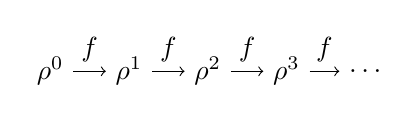
\begin{tikzpicture}
	\node (A) at (0,0) {$\rho^0$};
	\node (B) at (1,0) {$\rho^1$};
	\node (C) at (2,0) {$\rho^2$};
	\node (D) at (3,0) {$\rho^3$};
	\node (E) at (4,0) {$\ldots$};
	
	
	\draw[->] (A) -- node[above]{$f$} (B);
	\draw[->] (B) -- node[above]{$f$} (C);
	\draw[->] (C) -- node[above]{$f$} (D);
	\draw[->] (D) -- node[above]{$f$} (E);
\end{tikzpicture}
\end{center}

	\item \parbox[t]{\linewidth}{A sequence that ends in a cycle, meaning the sequence will repeat multiple states forever.\\
\begin{center}
	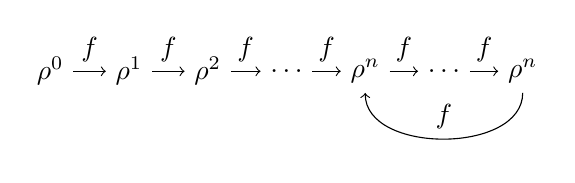
\begin{tikzpicture}
	\node (A) at (0,0) {$\rho^0$};
	\node (B) at (1,0) {$\rho^1$};
	\node (C) at (2,0) {$\rho^2$};
	\node (D) at (3,0) {$\ldots$};
	\node (E) at (4,0) {$\rho^n$};
	\node (F) at (5,0) {$\ldots$};
	\node (G) at (6,0) {$\rho^n$};
	
	
	\draw[->] (A) -- node[above]{$f$} (B);
	\draw[->] (B) -- node[above]{$f$} (C);
	\draw[->] (C) -- node[above]{$f$} (D);
	\draw[->] (D) -- node[above]{$f$} (E);
	\draw[->] (E) -- node[above]{$f$} (F);
	\draw[->] (F) -- node[above]{$f$} (G);
	
	\draw[->] (G) edge [in=-90, out=-90,looseness=1] node[above]{$f$} (E);
\end{tikzpicture}
\end{center}
}
	\item A sequence that ends in a fixpoint $\rho^n$, such that $f(\rho^n)=\rho^n$.\\
\begin{center}
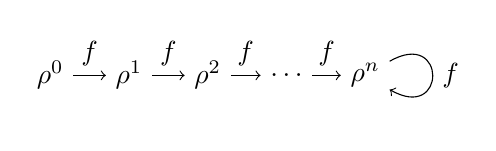
\begin{tikzpicture}
	\node (A) at (0,0) {$\rho^0$};
	\node (B) at (1,0) {$\rho^1$};
	\node (C) at (2,0) {$\rho^2$};
	\node (D) at (3,0) {$\ldots$};
	\node (E) at (4,0) {$\rho^n$};
	
	
	\draw[->] (A) -- node[above]{$f$} (B);
	\draw[->] (B) -- node[above]{$f$} (C);
	\draw[->] (C) -- node[above]{$f$} (D);
	\draw[->] (D) -- node[above]{$f$} (E);
	
	\draw[->] (E) edge [in=-30, out=30,looseness=6] node[right]{$f$} (E);
\end{tikzpicture}
\end{center}
\end{enumerate} 

\noindent Since we rely on the sequence to end in a fixpoint, so that we can end our abstract loop, we need to eliminate cases 1 and 2. For this we apply the widening operator $\triangledown$ after every loop pass. This operator is a function $\triangledown: \mathcal{R}_v\mapsto \mathcal{R}_v$, such that $f(\rho)\sqsubseteq\rho\triangledown f(\rho)$ and every infinite sequence $\rho^0,\rho^1,\dots$, where $\rho^n=\rho^{n-1}\triangledown f(\rho^{-1})$ is not strictly increasing \cite{cousot1977}. The exact definition of this widening operator depends on the used abstract domain.

\section{The Interval Domain}

\begin{figure}[!htb]
\begin{center}
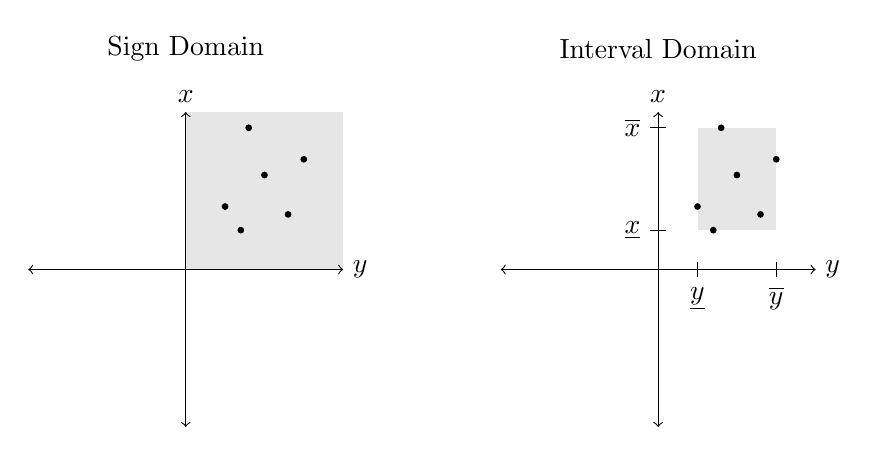
\begin{tikzpicture}
 		\coordinate (A) at (-1,-2);
		\coordinate (B) at (-1,2);
		\coordinate (C) at (-3,0);
		\coordinate (D) at (1,0);
		
		\draw [draw=none, fill=gray, fill opacity=0.2] (-1,0) -- (-1,2) -- (1,2) -- (1,0) -- cycle;
		
		%Axis
		\draw[<->] (A) -- (B) node [above] {$x$};
		\draw[<->] (C) -- (D) node [right] {$y$};
		
		
		\filldraw[black] (-0.5,0.8) circle (1pt);	
		\filldraw[black] (0,1.2) circle (1pt);
		\filldraw[black] (0.5,1.4) circle (1pt);	
		\filldraw[black] (-0.2,1.8) circle (1pt);
		\filldraw[black] (-0.3,0.5) circle (1pt);	
		\filldraw[black] (0.3,0.7) circle (1pt);	
		
		
		\node at (-1,2.8) {Sign Domain};
		
		\coordinate (E) at (5,-2);
		\coordinate (F) at (5,2);
		\coordinate (G) at (3,0);
		\coordinate (H) at (7,0);
		
		\draw [draw=none, fill=gray, fill opacity=0.2] (5.5,0.5) -- (5.5,1.8) -- (6.5,1.8) -- (6.5,0.5) -- cycle;
		
		\draw[-] (5.5,0.1) -- (5.5,-0.1);
		\draw[-] (6.5,0.1) -- (6.5,-0.1);
		
		\draw[-] (4.9,1.8) -- (5.1,1.8);
		\draw[-] (4.9,0.5) -- (5.1,0.5);
		
		\node at (5,1.8)[left, xshift=-1mm] {$\overline{x}$};
		\node at (5,0.5)[left, xshift=-1mm] {$\underline{x}$};
		
		\node at (5.5,0)[below, yshift=-1mm] {$\underline{y}$};
		\node at (6.5,0)[below, yshift=-1mm] {$\overline{y}$};
		
		%Axis
		\draw[<->] (E) -- (F) node [above] {$x$};
		\draw[<->] (G) -- (H) node [right] {$y$};
		
		\filldraw[black] (5.5,0.8) circle (1pt);	
		\filldraw[black] (6,1.2) circle (1pt);
		\filldraw[black] (6.5,1.4) circle (1pt);	
		\filldraw[black] (5.8,1.8) circle (1pt);
		\filldraw[black] (5.7,0.5) circle (1pt);	
		\filldraw[black] (6.3,0.7) circle (1pt);		
		
		\node at (5,2.8) {Interval Domain};		
		
		
\end{tikzpicture}
\end{center}
\caption{A diagram comparing abstract representation for a set of states. In this example a concrete state consists only of two scalar variable values $x$ and $y$. Therefore a concrete state can be represented as a point in the plane. The sign domain state, which is abstracting the marked concrete states, spans an entire quadrant of the coordinate system, whereas the interval domain state only occupies the rectangle encasing the states.}\label{fig:domaincomparison}
\end{figure}


\begin{figure}[htb]
	\begin{center}
		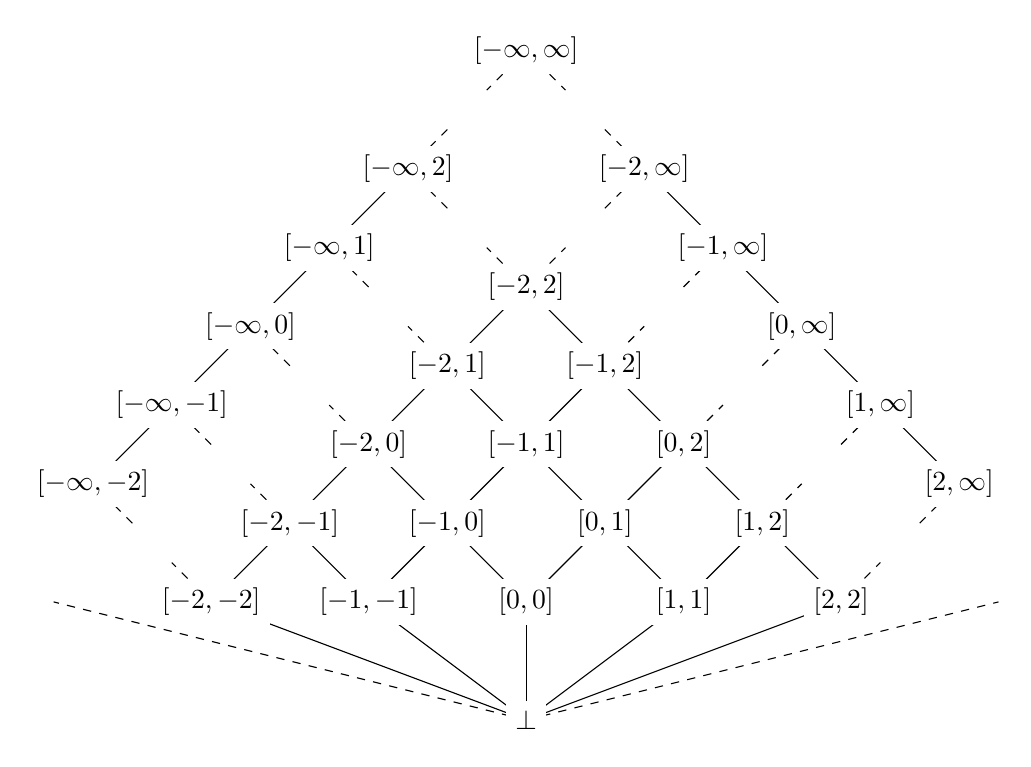
\begin{tikzpicture}
            \draw (0,0) -- (0,1.5);
            \draw (0,0) -- (2,1.5);
            \draw (0,0) -- (4,1.5);
            \draw (0,0) -- (-2,1.5);
            \draw (0,0) -- (-4,1.5);
            \draw (0,0)[dashed] -- (-6,1.5);
            \draw (0,0)[dashed] -- (6,1.5);
            
            \draw (2,1.5) -- (1,2.5);
            \draw (2,1.5) -- (3,2.5);
            \draw (4,1.5) -- (3,2.5);
            \draw (0,1.5) -- (1,2.5);
            \draw (0,1.5) -- (-1,2.5);
            \draw (-2,1.5) -- (-1,2.5);
            \draw (-2,1.5) -- (-3,2.5);
            \draw (-4,1.5) -- (-3,2.5);
            
            \draw (1,2.5) -- (0,3.5);
            \draw (1,2.5) -- (2,3.5);
            \draw (3,2.5) -- (2,3.5);
            \draw (-1,2.5) -- (0,3.5);
            \draw (-1,2.5) -- (-2,3.5);
            \draw (-3,2.5) -- (-2,3.5);
            
            \draw (2,3.5) -- (1,4.5);
            \draw (0,3.5) -- (1,4.5);
            \draw (0,3.5) -- (-1,4.5);
            \draw (-2,3.5) -- (-1,4.5);
            
            \draw (-1,4.5) -- (0,5.5);
            \draw (1,4.5) -- (0,5.5);
            
            \draw (-4,1.5)[dashed] -- (-4.5,2);
            \draw (-5,2.5)[dashed] -- (-5.5,3);
            
            \draw (-3,2.5)[dashed] -- (-3.5,3);
            \draw (-4,3.5)[dashed] -- (-4.5,4);
            
            \draw (-2,3.5)[dashed] -- (-2.5,4);
            \draw (-3,4.5)[dashed] -- (-3.5,5);
            
            \draw (-1,4.5)[dashed] -- (-1.5,5);
            \draw (-2,5.5)[dashed] -- (-2.5,6);
            
            \draw (0,5.5)[dashed] -- (-0.5,6);
            \draw (-1,6.5)[dashed] -- (-1.5,7);
           
            \draw (4,1.5)[dashed] -- (4.5,2);
            \draw (5,2.5)[dashed] -- (5.5,3);
            
            \draw (3,2.5)[dashed] -- (3.5,3);
            \draw (4,3.5)[dashed] -- (4.5,4);
            
            \draw (2,3.5)[dashed] -- (2.5,4);
            \draw (3,4.5)[dashed] -- (3.5,5);
            
            \draw (1,4.5)[dashed] -- (1.5,5);
            \draw (2,5.5)[dashed] -- (2.5,6);
            
            \draw (0,5.5)[dashed] -- (0.5,6);
            \draw (1,6.5)[dashed] -- (1.5,7);
            
            \draw (-5.5,3) -- (-1.5,7);
            \draw (5.5,3) -- (1.5,7);
            
            \draw (-1,7.5)[dashed] -- (-1.5,7);
            \draw (1,7.5)[dashed] -- (1.5,7);
            
            \draw (0,8.5)[dashed] -- (-0.5,8);
            \draw (0,8.5)[dashed] -- (0.5,8);
            
            \draw (0,0) node[fill=white!5] {$\perp$};
            \draw (0,1.5) node[fill=white!5] {$[0,0]$};
            \draw (2,1.5) node[fill=white!5] {$[1,1]$};
            \draw (4,1.5) node[fill=white!5] {$[2,2]$};
            \draw (-2,1.5) node[fill=white!5] {$[-1,-1]$};
            \draw (-4,1.5) node[fill=white!5] {$[-2,-2]$};
            
            \draw (1,2.5) node[fill=white!5] {$[0,1]$};
            \draw (3,2.5) node[fill=white!5] {$[1,2]$};
            \draw (-1,2.5) node[fill=white!5] {$[-1,0]$};
            \draw (-3,2.5) node[fill=white!5] {$[-2,-1]$};
            
            \draw (2,3.5) node[fill=white!5] {$[0,2]$};
            \draw (0,3.5) node[fill=white!5] {$[-1,1]$};
            \draw (-2,3.5) node[fill=white!5] {$[-2,0]$};
            
            \draw (1,4.5) node[fill=white!5] {$[-1,2]$};
            \draw (-1,4.5) node[fill=white!5] {$[-2,1]$};
            
            \draw (0,5.5) node[fill=white!5] {$[-2,2]$};
            
            
            \draw (-5.5,3) node[fill=white!5] {$[-\infty,-2]$};
            \draw (-4.5,4) node[fill=white!5] {$[-\infty,-1]$};
            \draw (-3.5,5) node[fill=white!5] {$[-\infty,0]$};
            \draw (-2.5,6) node[fill=white!5] {$[-\infty,1]$};
            \draw (-1.5,7) node[fill=white!5] {$[-\infty,2]$};
            
            
            \draw (5.5,3) node[fill=white!5] {$[2,\infty]$};
            \draw (4.5,4) node[fill=white!5] {$[1,\infty]$};
            \draw (3.5,5) node[fill=white!5] {$[0,\infty]$};
            \draw (2.5,6) node[fill=white!5] {$[-1,\infty]$};
            \draw (1.5,7) node[fill=white!5] {$[-2,\infty]$};
            
            \draw (0,8.5) node[fill=white!5] {$[-\infty,\infty]$};
         
        \end{tikzpicture}
        \caption{The interval abstract domain as a Hasse diagram \cite{cousot1977}}.\label{fig:intervaldomain}
	\end{center}
\end{figure}

Until this point, we have been doing our abstract interpretation in the sign domain only. Let us introduce another, more precise one: The interval domain. This domain does not abstract the sign property of a scalar variable, but rather the property of which interval it is included in. An interval $[\underline{x},\overline{x}]$ has the concretisation $\gamma([\underline{x},\overline{x}])=\{z\in\mathbb{Z} \;|\; \underline{x}\leq z \leq \overline{x}\}$. Abstract expression operations follow usual interval arithmetics. For example, $[\underline{x},\overline{x}]+[\underline{y},\overline{y}]=[\underline{x}+\underline{y},\overline{x}+\overline{y}]$. Figure \ref{fig:domaincomparison} compares the sign domain to the interval domain and shows graphically how it abstracts in a more precise manner. Figure \ref{fig:intervaldomain} shows the interval lattice as a Hasse diagram.

\clearpage \section{The FunArray}

\subsection{Abstract Array Segmentation Predicates}

A FunArray predicate, as depicted in figure \ref{fig:funarraypredicate}, takes the form \funArray{\bound{e_1^1\ldots e_{m^1}^1} \fvalue{P_1} \bound{e_1^2\ldots e_{m^2}^2}[?^2] \fvalue{P_2}\ldots\allowbreak\fvalue{P_{n-1}}\allowbreak \bound{e_1^n\ldots e_{m^n}^n}[?^n]}, where $e^i_1\ldots e^i_m\in\mathbb{E}$ are expressions in normal form determining segment bounds, $P_i\in A$ are abstract element values from a chosen abstract domain $A$ and the optional $[?_i]$ signifies whether a preceding segment might be possibly empty \cite{cousot2011}. The FunArray maintains the condition that $e_1^1=\ldots=e_{m^1}^1\leq e_1^2=\ldots=e_{m^2}^2\leq\ldots\leq e_1^n=\ldots=e_{m^n}^n$, meaning that expressions in the same bound evaluate to an equal value and that the bounds are ordered. 
\vspace{0.2cm}
\begin{figure}[!htb]
\begin{center}
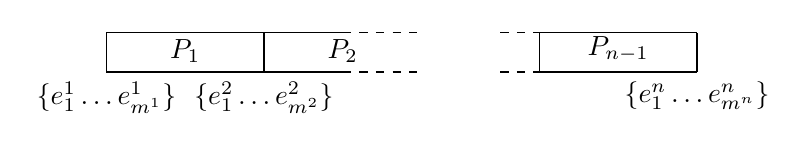
\begin{tikzpicture}

	\draw (0,0) -- (0,0.5);
	\draw (0,0) -- node[above]{$P_1$} (2,0);
	\draw (0,0.5) -- (2,0.5);
	\node[below] at (0,0) {$\{e_1^1\ldots e_{m^1}^1\}$};
	
	\draw (2,0) -- (2,0.5);
	\draw (2,0) -- node[above, xshift=0.5cm]{$P_2$} (3,0);
	\draw (2,0.5) -- (3,0.5);
	\node[below] at (2,0) {$\{e_1^2\ldots e_{m^2}^2\}$};
	\draw[dashed] (3,0) -- (4,0);
	\draw[dashed] (3,0.5) -- (4,0.5);
	
	
	\draw[dashed] (5,0) -- (5.5,0);
	\draw[dashed] (5,0.5) -- (5.5,0.5);
	\draw (5.5,0) -- (5.5,0.5);
	\draw (7.5,0) -- (7.5,0.5);
	\draw (5.5,0) -- node[above]{$P_{n-1}$} (7.5,0);
	\draw (5.5,0.5) -- (7.5,0.5);
	
	\node[below] at (7.5,0) {$\{e_1^n\ldots e_{m^n}^n\}$};
\end{tikzpicture}
\end{center}
\caption{Graphical representation of a the FunArray predicate.}
\end{figure}

\noindent Consider the following predicate for example: \funArray{A: \bound{0 \;\; a} \fvalue{[0,10]} \bound{a +4} \fvalue{[0,0]} \bound{b}?}. This means that the array $A$ has two segments. The first one which is bound by the expressions $0$ and $a$ on its left side and by $a+4$ on its right side. All array accesses with an index $i$ with $0=a\leq i \leq a+ 4$ will return the abstract value $[0,10]$. The second segment is bound by $a+4$ and $b$. It has the value $[0,0]$ and might possibly be empty as signified by the question mark.


\subsection{Functors}

An abstract domain functor is a function from the parameter domains $D_1,\ldots,D_n$ to a new abstract domain $D(D_1,\ldots,D_n)$ \cite{cousot2011}.
Since the FunArray is a functor $S(B(E),A,R)$, it can be adapted to a wide range of analyses by tweaking its parameter domains. It takes the following domains as arguments:
\begin{itemize}[label={--}]
	\item The segment bound $B(E)$, which in turn is also a functor from the expression domain $E$.
	\item The array element abstract domain $A$. This is an arbitrary abstraction on the examined values. In the remaining examples in this thesis, this is going to be the interval domain.
	\item The variable abstract domain $R$.
\end{itemize} 

\subsection{Abstract operations}

As an abstract domain, the FunArray supports the abstract operations join $\sqcup$, meet $\sqcap$, partial order $\sqsubseteq$, widen $\triangledown$ and narrow $\vartriangle$. To apply these, the segment bounds of the triangle need to be unified and the respective operation applied segment wise. Unification is a process whereby the FunArrays $A$ and $B$ are modified into $A'$ and $B'$, such that $A\sqsubseteq A'$ and $B\sqsubseteq B'$ and the segment bounds for $A'$ and $B'$ are identical.


\subsection{Transformers}

An array access \texttt{A[e]} in the FunArray domain is not as trivial as in a concrete execution of a program. Because \texttt{e} might not actually be present in the bounds of the FunArray, we need to find the greatest bound $B_l\leq \llbracket \texttt{e}\rrbracket$ and the least bound $B_g\geq \llbracket \texttt{e}\rrbracket$ in a given array. The evaluation of the array access is then $\llbracket\texttt{A[e]}\rrbracket=\bigsqcup^{g-1}_{k=l}P_k$.

An array is modified by the array assignment \texttt{A[i] = e}. Its semantics is defined as follows: $\llbracket\texttt{A[i] = e}\rrbracket\rho=\rho[A:=A']$, meaning the array $A: B_1P_1B_2[?_1]\ldots P_{n-1}\allowbreak{}B_n[?_{n-1}]$ has been replaced by the modified $A': B_1P_1B_2[?_1]\ldots\allowbreak B_l[?_l] (\bigsqcup^{g-1}_{k=l}P_k)\allowbreak\, \{\,\llbracket\texttt{i}\rrbracket\,\}?\, \llbracket\texttt{e}\rrbracket \allowbreak\,\{\,\llbracket\texttt{i}\rrbracket+1\,\}\, \allowbreak(\bigsqcup^{g-1}_{k=l}P_k) B_g?\ldots \allowbreak P_{n-1}B_n[?_{n-1}]$, whereby $B_l\leq\llbracket\texttt{i}\rrbracket\leq B_g$.

When modifying variables in the state, the FunArray predicates also need to be modified as they might contain that variable. Consider an array \funArray{A: \bound{a} \fvalue{P_1} \bound{b} \fvalue{P_2} \bound{c}}. If there is an assignment \texttt{b := b+1}, the FunArray needs to be modified to \funArray{A': \bound{a} \fvalue{P_1} \bound{b-1} \fvalue{P_2} \bound{c}}, so that it is still correct. 















